\let\negmedspace\undefined
\let\negthickspace\undefined
\documentclass[journal]{IEEEtran}
\usepackage[a5paper, margin=10mm, onecolumn]{geometry}
%\usepackage{lmodern} % Ensure lmodern is loaded for pdflatex
\usepackage{tfrupee} % Include tfrupee package

\setlength{\headheight}{1cm} % Set the height of the header box
\setlength{\headsep}{0mm}     % Set the distance between the header box and the top of the text

\usepackage{gvv-book}
\usepackage{gvv}
\usepackage{cite}
\usepackage{amsmath,amssymb,amsfonts,amsthm}
\usepackage{algorithmic}
\usepackage{graphicx}
\usepackage{textcomp}
\usepackage{xcolor}
\usepackage{txfonts}
\usepackage{listings}
\usepackage{enumitem}
\usepackage{mathtools}
\usepackage{gensymb}
\usepackage{comment}
\usepackage[breaklinks=true]{hyperref}
\usepackage{tkz-euclide} 
\usepackage{listings}
% \usepackage{gvv}                                        
\def\inputGnumericTable{}                                 
\usepackage[latin1]{inputenc}                                
\usepackage{color}                                            
\usepackage{array}                                            
\usepackage{longtable}                                       
\usepackage{calc}                                             
\usepackage{multirow}                                         
\usepackage{hhline}                                           
\usepackage{ifthen}
\usepackage{lscape}
\begin{document}

\bibliographystyle{IEEEtran}



\title{4.7.54}
\author{EE25BTECH11057 - Rushil Shanmukha Srinivas
}
% \maketitle
% \newpage
% \bigskip
{\let\newpage\relax\maketitle}

\renewcommand{\thefigure}{\theenumi}
\renewcommand{\thetable}{\theenumi}
\setlength{\intextsep}{10pt} % Space between text and floats

\numberwithin{equation}{enumi}
\numberwithin{figure}{enumi}
\renewcommand{\thetable}{\theenumi}

\textbf{Problem:} Find the vector equations of the line passing through the point (1,2,-4) and 
perpendicular to the two lines 

$\frac{x-8}{3} = \frac{y+19}{-16} = \frac{z-10}{7}$ and
$\frac{x-15}{3} = \frac{y-29}{8} = \frac{z-5}{-5}$.

\textbf{Solution:} Given the line passes through the point
\begin{align}
\vec{A} = \myvec{1\\2\\-4}
\end{align}
The line is also perpendicular to
\begin{align}
\frac{x-8}{3} = \frac{y+19}{-16} = \frac{z-10}{7} ,
\frac{x-15}{3} = \frac{y-29}{8} = \frac{z-5}{-5}.
\end{align}
The direction vector of the line is given by
\begin{align}
\myvec{
3 & -16 & 7 \\
3 & 8 & -5} \vec{m} = 0 \xleftrightarrow{R_2\longrightarrow R_2-R_1}
\myvec{
3 & -16 & 7 \\
0 & 24 & -12}
\end{align}
\begin{align}
\myvec{
3 & -16 & 7 \\
0 & 24 & -12} \xleftrightarrow{R_1\longrightarrow 3R_1+2R_2}
\myvec{
9 & 0 & -3 \\
0 & 24 & -12}
\end{align}
\begin{align}
\myvec{
9 & 0 & -3 \\
0 & 24 & -12} \xleftrightarrow{R_1\longrightarrow \frac{R_1}{9}}
\myvec{
1 & 0 & \frac{-1}{3} \\
0 & 24 & -12}
\end{align}
\begin{align}
\myvec{
1 & 0 & \frac{-1}{3} \\
0 & 24 & -12} \xleftrightarrow{R_2\longrightarrow \frac{R_2}{24}}
\myvec{
1 & 0 & \frac{-1}{3} \\
0 & 1 & \frac{-1}{2}} 
\end{align}
So \begin{align}
\vec{m}=\myvec{2\\3\\6} = Direction \ vector \ of \ line
\end{align}
The vector equation of the line is
\begin{align}
\vec{L_1} = \vec{A}+k\vec{m} = \myvec{1\\2\\-4}+k\myvec{2\\3\\6}
\end{align}

\begin{figure}[h!]
  \centering
  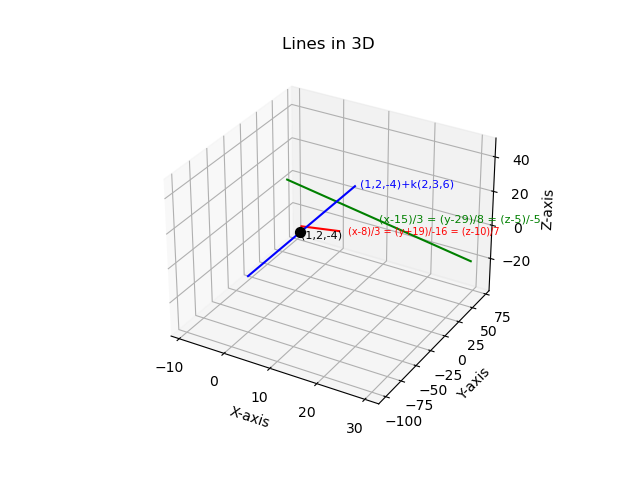
\includegraphics[width=0.9\columnwidth]{figs/fig7.png} 
   \caption*{Fig: Representation of Lines and Point}
  \label{Fig7}
\end{figure}

\end{document}